\documentclass[11pt,landscape]{article}
\usepackage{multicol}
\usepackage{calc}
\usepackage{ifthen}
\usepackage[landscape]{geometry}
\usepackage{hyperref}
\usepackage{amsmath}
\usepackage{graphicx}
\usepackage{float}

% To make this come out properly in landscape mode, do one of the following
% 1.
%  pdflatex latexsheet.tex
%
% 2.
%  latex latexsheet.tex
%  dvips -P pdf  -t landscape latexsheet.dvi
%  ps2pdf latexsheet.ps


% If you're reading this, be prepared for confusion.  Making this was
% a learning experience for me, and it shows.  Much of the placement
% was hacked in; if you make it better, let me know...


% To Do:
% \listoffigures \listoftables
% \setcounter{secnumdepth}{0}


% This sets page margins to .5 inch if using letter paper, and to 1cm
% if using A4 paper. (This probably isn't strictly necessary.)
% If using another size paper, use default 1cm margins.
\ifthenelse{\lengthtest { \paperwidth = 11in}}
	{ \geometry{top=.5in,left=.5in,right=.5in,bottom=.5in} }
	{\ifthenelse{ \lengthtest{ \paperwidth = 297mm}}
		{\geometry{top=1cm,left=1cm,right=1cm,bottom=1cm} }
		{\geometry{top=1cm,left=1cm,right=1cm,bottom=1cm} }
	}

% Turn off header and footer
\pagestyle{empty}
 

% Redefine section commands to use less space
\makeatletter
\renewcommand{\section}{\@startsection{section}{1}{0mm}%
                                {-1ex plus -.5ex minus -.2ex}%
                                {0.5ex plus .2ex}%x
                                {\normalfont\large\bfseries}}
\renewcommand{\subsection}{\@startsection{subsection}{2}{0mm}%
                                {-1explus -.5ex minus -.2ex}%
                                {0.5ex plus .2ex}%
                                {\normalfont\normalsize\bfseries}}
\renewcommand{\subsubsection}{\@startsection{subsubsection}{3}{0mm}%
                                {-1ex plus -.5ex minus -.2ex}%
                                {1ex plus .2ex}%
                                {\normalfont\small\bfseries}}
\makeatother

% Define BibTeX command
\def\BibTeX{{\rm B\kern-.05em{\sc i\kern-.025em b}\kern-.08em
    T\kern-.1667em\lower.7ex\hbox{E}\kern-.125emX}}

% Don't print section numbers
\setcounter{secnumdepth}{0}


\setlength{\parindent}{0pt}
\setlength{\parskip}{0pt plus 0.5ex}


% -----------------------------------------------------------------------

\begin{document}

\raggedright
\footnotesize
\begin{multicols}{3}


% multicol parameters
% These lengths are set only within the two main columns
%\setlength{\columnseprule}{0.25pt}
\setlength{\premulticols}{1pt}
\setlength{\postmulticols}{1pt}
\setlength{\multicolsep}{1pt}
\setlength{\columnsep}{2pt}

\begin{center}
     \Large{\textbf{EECS 301 Cheat Sheet}} \\
\end{center}

\section{Definitions}
${n\choose k} = \dfrac{n!}{r!(n-r)!} = {n\choose n-k}$ \\
$P(A\vert B) = \dfrac{P(A\cap B)}{P(B)}$ \\
$P\{X = k\} = {N\choose k}p^k (1-p)^{1-k}$ \\
Independent if $P(A\cap B) = P(A)P(B)$ \\
Expected Value = $\sum^\infty_{k=0}kP\{X=k\}$



\section{Conditional Probability}
$P(\bar{B}\vert A) = 1 - P(B\vert A)$ \\
$P(B\cup C\vert A) = P(B\vert A) + P(C\vert A) - P((B\cap C)\vert A)$ \\
$P(B\vert A) = \dfrac{P(A\vert B)P(B)}{P(A)}$ \\
$P(B) = P(B\vert A)P(A) + P(B\vert\bar{A})P(\bar{A})$ \\
$P(A\cap B\cap C) = P(C\vert A\cap B)P(B\vert A)P(A)$ 


\subsection{Binomial}
$\sum^N_{k = 0}{N\choose k}p^k q^{N-k} = (p+q)^N$ \\
$\sum^N_{k = 0}{N\choose k}r^k = (1+r)^N$ \\
$\sum^{b}_{k=a} r^{k} = \dfrac{r^a - r^{b+1}}{1-r}$ \\
$\sum^{\infty}_{k=0} kr^{k} = \dfrac{r}{(r-1)^2}$

%---------------------------------------------------------------------------

\end{multicols}

\begin{multicols}{3}
\setlength{\premulticols}{1pt}
\setlength{\postmulticols}{1pt}
\setlength{\multicolsep}{1pt}
\setlength{\columnsep}{2pt}

\begin{figure}[H]
    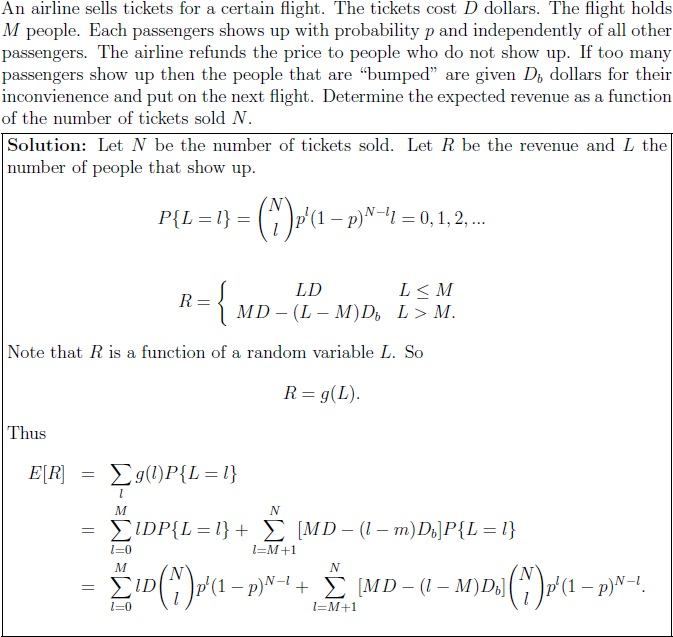
\includegraphics[scale=0.46]{./Images/1/Airplanes.jpg}
\end{figure}
\begin{figure}[H]
    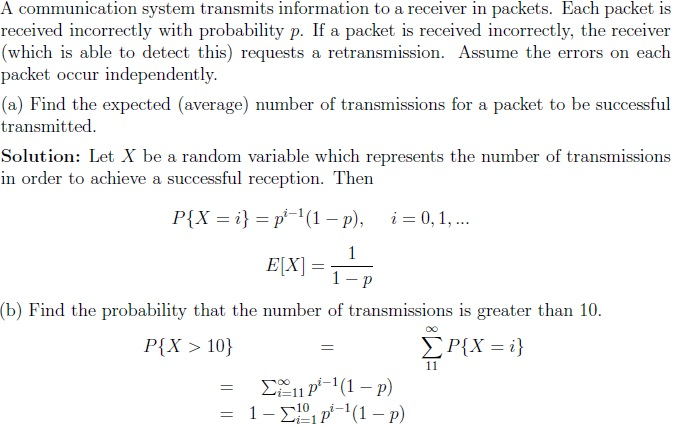
\includegraphics[scale=0.46]{./Images/1/Communication.jpg}
\end{figure}
\begin{figure}[H]
    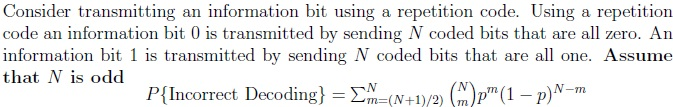
\includegraphics[scale=0.46]{./Images/1/HammingCode.jpg}
\end{figure}
\begin{figure}[H]
    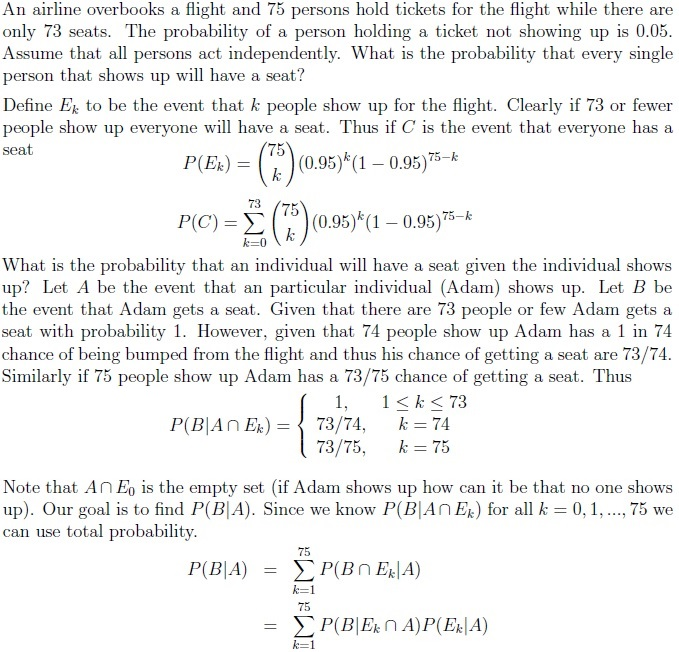
\includegraphics[scale=0.46]{./Images/1/Seat1.jpg}
    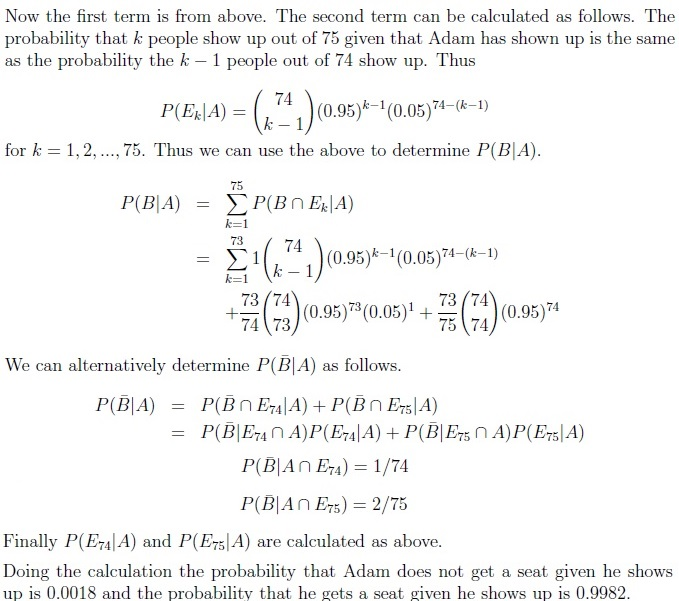
\includegraphics[scale=0.46]{./Images/1/Seat2.jpg}
\end{figure}
\begin{figure}[H]
    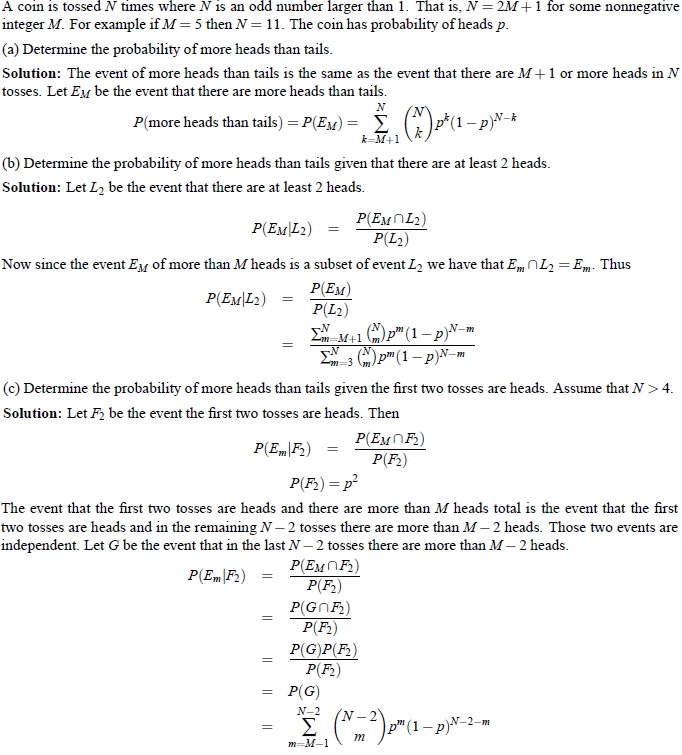
\includegraphics[scale=0.46]{./Images/1/Cointoss.jpg}
\end{figure}
\begin{figure}[H]
    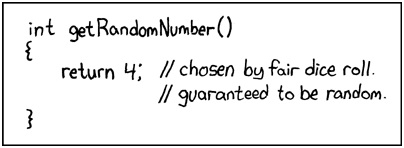
\includegraphics[scale=0.8]{./Images/1/RandNumXKCD.jpg}
\end{figure}
\end{multicols}

\end{document}
